\section{Fouriertransformation}
Mithilfe der Fouriertransformierten kann ein endliches nicht periodisches Signal analysiert werden. Dazu wechselt man vom Zeitbereich in den Frequenzbereich.\\
\begin{tabular}{|l|l|}
	\hline \textbf{Fourierintegral} & $F(j\omega) = \int\limits_{-\infty}^{\infty} f(t)e^{-j\omega t}dt$\\
	\hline \textbf{Rücktransformierte} &$\frac{1}{2\pi}\int\limits_{-\infty}^{\infty}
	F(j\omega)e^{j\omega t}d\omega$\\
	\hline
\end{tabular}

\subsection{Eigenschaften der Fouriertransformierten}
\begin{tabular}{|l|l|}
	\hline
	Linearität & 
	$\alpha\cdot f(t) + \beta\cdot g(t) \;\laplace\;\alpha\cdot F(j\omega) +
	\beta\cdot G(j\omega)$\\
	\hline
	Zeitumkehrung (Spiegelung an der Y-Achse)&
	$f(-t) \;\laplace\; F(-j\omega) = F^*(jw)$ \\
	\hline        	
	Streckung im Zeitbereich &
	$f(\alpha t) \;\laplace\; \frac{1}{|\alpha|}F \left (j\frac{\omega}{\alpha} \right)
	\quad\alpha \in\mathbb{R}\setminus \{0\}$\\
	\hline
	Verschiebung im	Zeitbereich &
	$f(t\pm t_0) \;\laplace\; F(j\omega)e^{\pm j\omega t_0}$\\
	\hline
	Verschiebung im Frequenzbereich &
	$f(t)e^{\pm j\omega_0 t} \;\laplace\; F(j(\omega\mp\omega_0))$\\
	\hline
	Ableitung im Zeitbereich &
	$\frac{\partial^n f(t)}{\partial t^n} \;\laplace\; (j\omega)^n F(j\omega)$\\
	\hline
	Integration im Zeitbereich &
	$\int\limits_{-\infty}^{t}f(\tau)d\tau \;\laplace\;
	\frac{F(j\omega)}{j\omega}+F(0)\pi\delta(\omega)$\\
	\hline				
	Ableitung im Frequenzbereich &
	$t^n f(t) \;\laplace\; j^n \frac{\partial F(j\omega)}{\partial \omega^n}$\\
	\hline		
	Faltung im Zeitbereich &
	$f(t) \ast g(t) = \int\limits_{-\infty}^{\infty} f(\tau)g(t-\tau)d\tau \;\laplace\;
	F(j\omega) \cdot G(j\omega)$\\
	\hline
	Faltung im Frequenzbereich &
	$f(t) \cdot g(t) \;\laplace\; \frac{1}{2\pi}F(j\omega) \ast G(j\omega)$\\
	\hline
	Vertauschungssatz (Dualität) &
	$f(t) \;\laplace\; F(j\omega)\nonumber$ \\
	& $F(t) \;\Laplace\; 2\pi \cdot f(-j\omega)$\\
	\hline
	Modulation &
	$\cos(\alpha t) \cdot f(t)  \;\laplace\;  \frac{1}{2}\cdot
	\left[F(j(\omega-\alpha)) + F(j(\omega+\alpha))\right ]$\\
	& $\sin(\alpha t) \cdot f(t) \;\laplace\; \frac{1}{2j}\cdot \left[
	F(j(\omega-\alpha)) - F(j(\omega+\alpha))\right ]$\\
	\hline
	Parseval's Theorem &
	$\int\limits_{-\infty}^{\infty}f(t)g^{\ast}(t)dt = \frac{1}{2\pi}
	\int\limits_{-\infty}^{\infty}F(j\omega)G^{\ast}(j\omega)d\omega$\\
	\hline
	Bessel's Theorem &
	$\int\limits_{-\infty}^{\infty}|f(t)|^2 dt = \frac{1}{2\pi}
	\int\limits_{-\infty}^{\infty}|F(j\omega)|^2 d\omega$\\
	\hline 			
	Anfangswerte &
	$f(0)=\frac{1}{2\pi}\int\limits_{-\infty}^{\infty}F(j\omega)d\omega
	\hspace*{1cm} F(0)=\int\limits_{-\infty}^{\infty}f(t)dt$\\
	\hline
	$\infty$ lange Folge von $\delta$-Impulsen &
	$\sum_{n=-\infty}^{\infty} \delta(t-n\cdot t_0) \;\laplace\;
	\sum_{n=-\infty}^{\infty} \frac{2\pi}{t_0}\delta(\omega-n\cdot
	\frac{2\pi}{t_0})$\\
	\hline
\end{tabular}
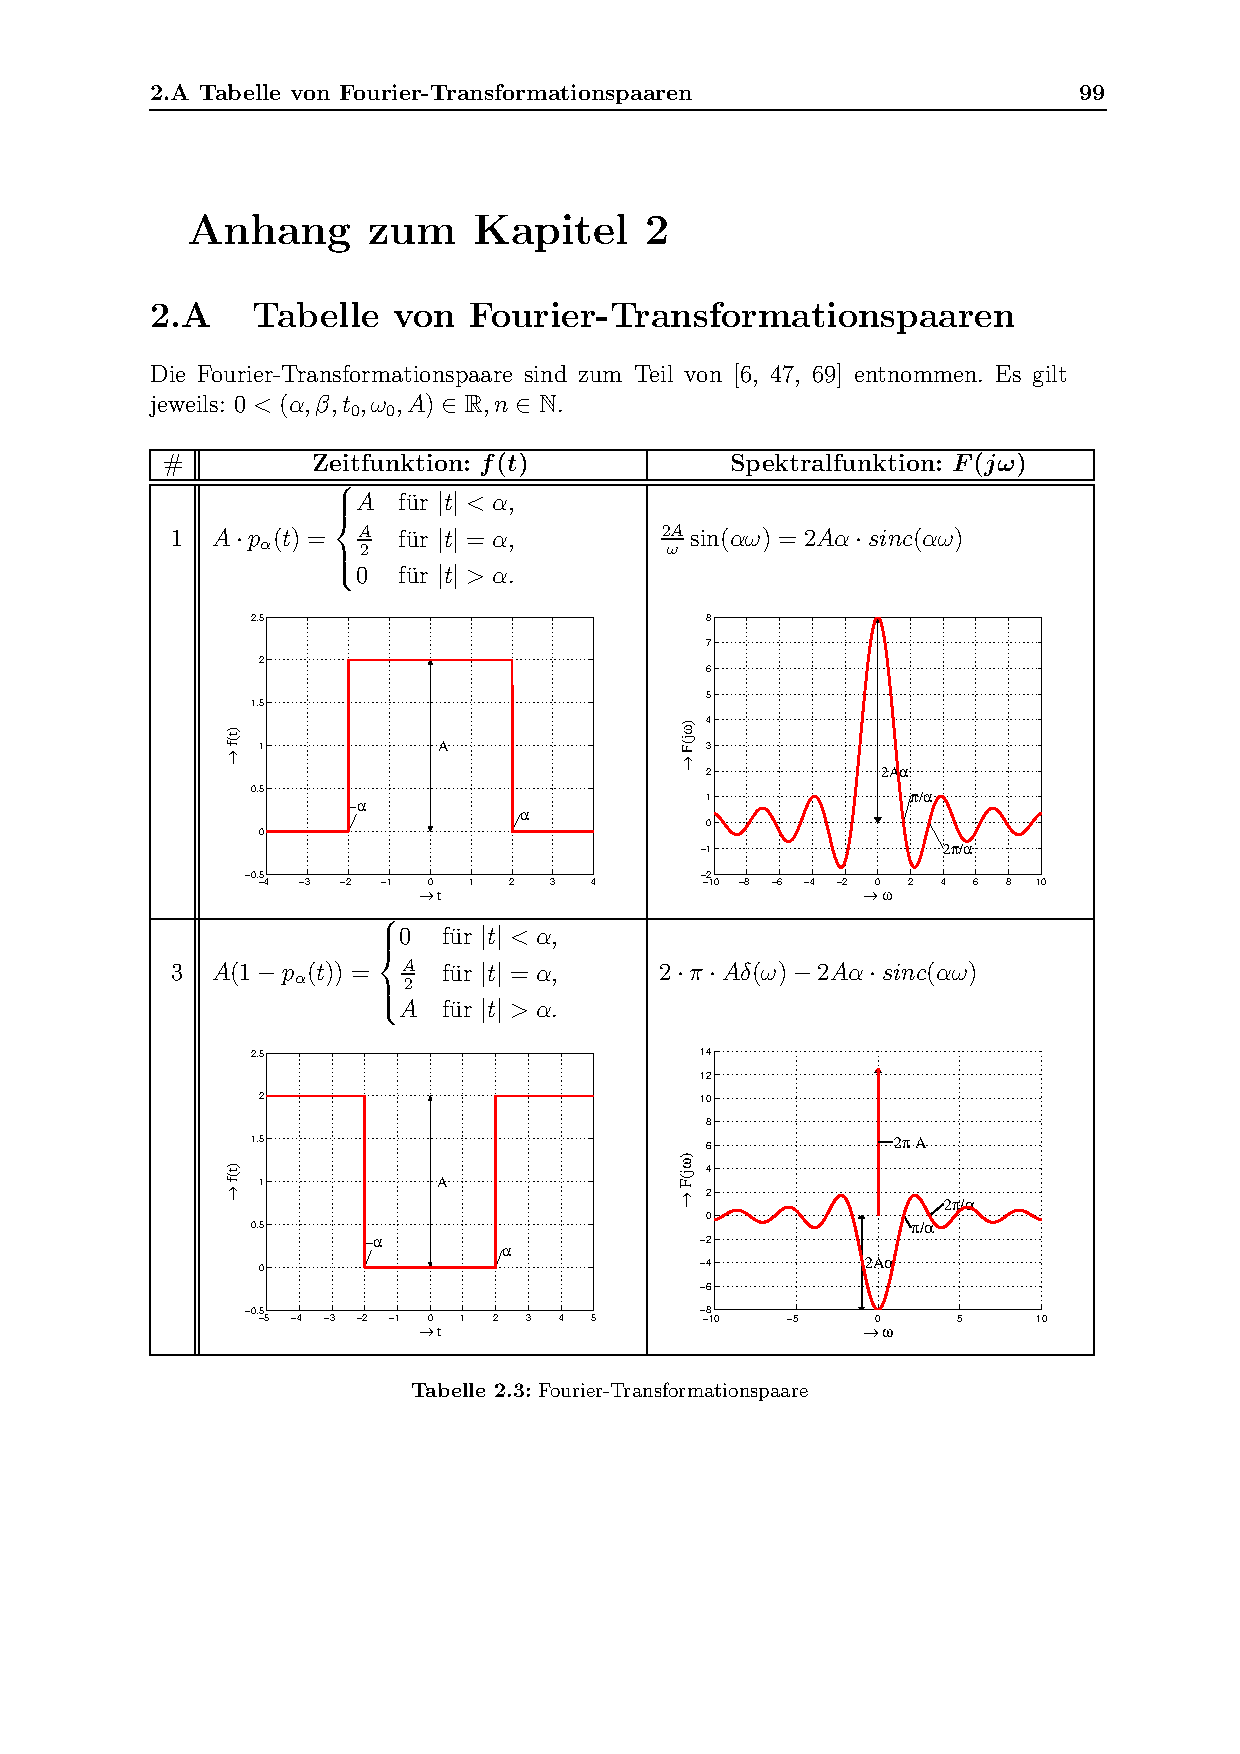
\includepdf[pages={1-7},pagecommand={},,scale=0.99]{sections/Tabellen.pdf}
\clearpage
\pagebreak